% !TEX program = xelatex
\documentclass[12pt]{article}
\usepackage[margin=1in]{geometry}
\usepackage{nopageno} % no page numbers
\usepackage{setspace} \doublespacing

\usepackage{graphicx}
\graphicspath{ {./graphics/} }
\usepackage[dvipsnames]{xcolor}
\definecolor{CrispBlue}{HTML}{0176AE}

\usepackage{fontspec}
\usepackage{tcolorbox}
\usepackage{etoolbox}
\BeforeBeginEnvironment{verbatim*}{\begin{tcolorbox}[colback=CrispBlue!5!white,colframe=CrispBlue!75!black]}%
\AfterEndEnvironment{verbatim*}{\end{tcolorbox}}%

\usepackage{hyperref}
\hypersetup{
    colorlinks,
    citecolor=black,
    filecolor=black,
    linkcolor=black,
    urlcolor=black
}

\renewcommand{\footnotesize}{\fontsize{8pt}{10pt}\selectfont}


\usepackage[labelfont={small,sc,bf},textfont={small,sc,bf}]{caption}
\setlength{\parindent}{24pt}
% \setlength{\parskip}{1em}

\usepackage{tocloft}
\renewcommand{\cftpartleader}{\cftdotfill{\cftdotsep}}
\renewcommand{\cftsecleader}{\cftdotfill{\cftdotsep}}

\usepackage[shortlabels]{enumitem}

\usepackage{lastpage}
\usepackage{fancyhdr}
\pagestyle{fancy}
\fancyhf{}
\renewcommand{\headrulewidth}{0pt}
\rfoot{Page \thepage\ of \pageref*{LastPage}}

\usepackage{amsmath,amsfonts,amssymb}
\usepackage{bm}
\usepackage{mathtools}

\renewcommand{\listfigurename}{List of Figures}

\begin{document}
\setmainfont{SF Pro Text}
\setsansfont{SF Pro Text}
\setmonofont{SF Mono}
\renewcommand{\familydefault}{\sfdefault}

\hypersetup{
    linkcolor=CrispBlue,
    urlcolor=CrispBlue,
    breaklinks=true
}

\noindent David Kirby\\
ECE 595: Mobile Edge Computing \& Networking\\
Spring 2022
\begin{center}
    \large\bfseries Assignment \#1
\end{center}

This assignment,


% \begin{figure}[!ht]
%     \centering
%     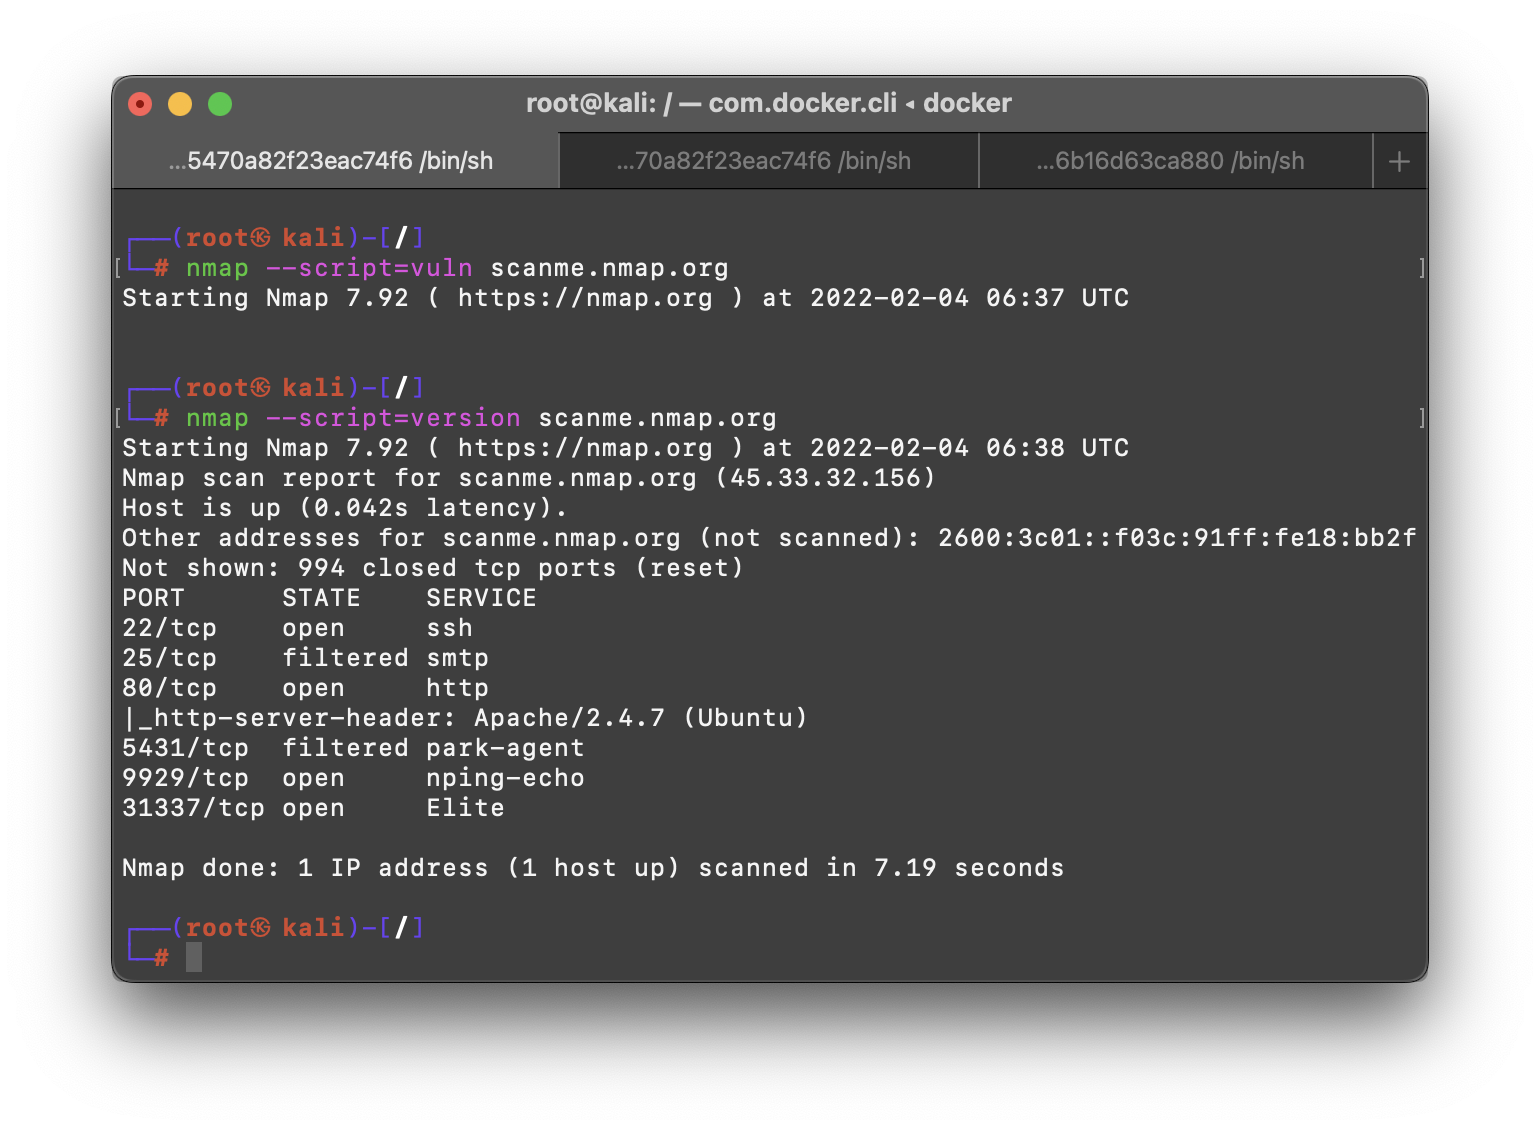
\includegraphics[width=0.8\textwidth]{figure10.png}\vspace{-1em}
%     \caption{Command line for nmap with scripts of scanme.nmap.org.}
%     \label{fig:nmap06}
% \end{figure}


\end{document}